\chapter{Test af reverb og echo impulsrespons}\label{sec:test_af_effekt}
Da echo og reverb begge er tidsinvariante effekter betyder det, at de kan karakteriseres af deres impulsrespons.\newline
Testens formål er at finde impulsresponset for echo- og reverbeffekten.
%Systemet består af modtager af indgangssignal, anti-aliasing filtre, TIVA-kit med EMP board, DAC, rekonstruktionsfilter og udgangskredsløbet.
Systemet består af et signalindgangs board, en række anti-aliasing og input filtre, et TIVA-kit med EMP board, et board med en DAC, nogle rekonstruktionsfilter og et udgangskredsløbet.
\section{Forsøgsopstilling og fremgangsmetode}
\begin{itemize}
	\item Funktionsgenerator sat på pulse med en peak-to-peak spænding sat til $500\si{mV}$ og et DC-offset sat til $250\si{mV}$ og pulsen sættes til at være $25\si{\mu S}$ lang svarende til en sample
	\item Oscilloskop sat til single sweep med en trigger sat til $200\si{mV}$
	\item Load modstand koblet på udgangen på $10\si{k\Omega}$
	\item Reverb delay sat til $10\si{mS}$ og input- og feedbackgain sat til $-0.50$
	\item Echo delay sat til $44\si{mS}$ samples og gain sat til $0.5$
\end{itemize}
%Funktionsgeneratoren kobles på signalindgangen af systemet, og oscilloskopets prober placeres hhv. på indgangen til mikrocontrolleren og på udgangen af rekonstruktionsfilteret.\newline
Funktionsgeneratoren kobles på signalindgangen sammen med en af oscilloskopets prober, den anden placeres udgangskredsløbet.\newline
Effektmodulerne aktiveres hver for sig og der tages et single sweep.
\subsection{Resultat}
Inputtet er den første impuls angivet som den gule graf og outputtet er vist ved den røde graf:
\begin{figure}[!ht]
		\centering
	\begin{minipage}{0.50\textwidth}
		\centering
		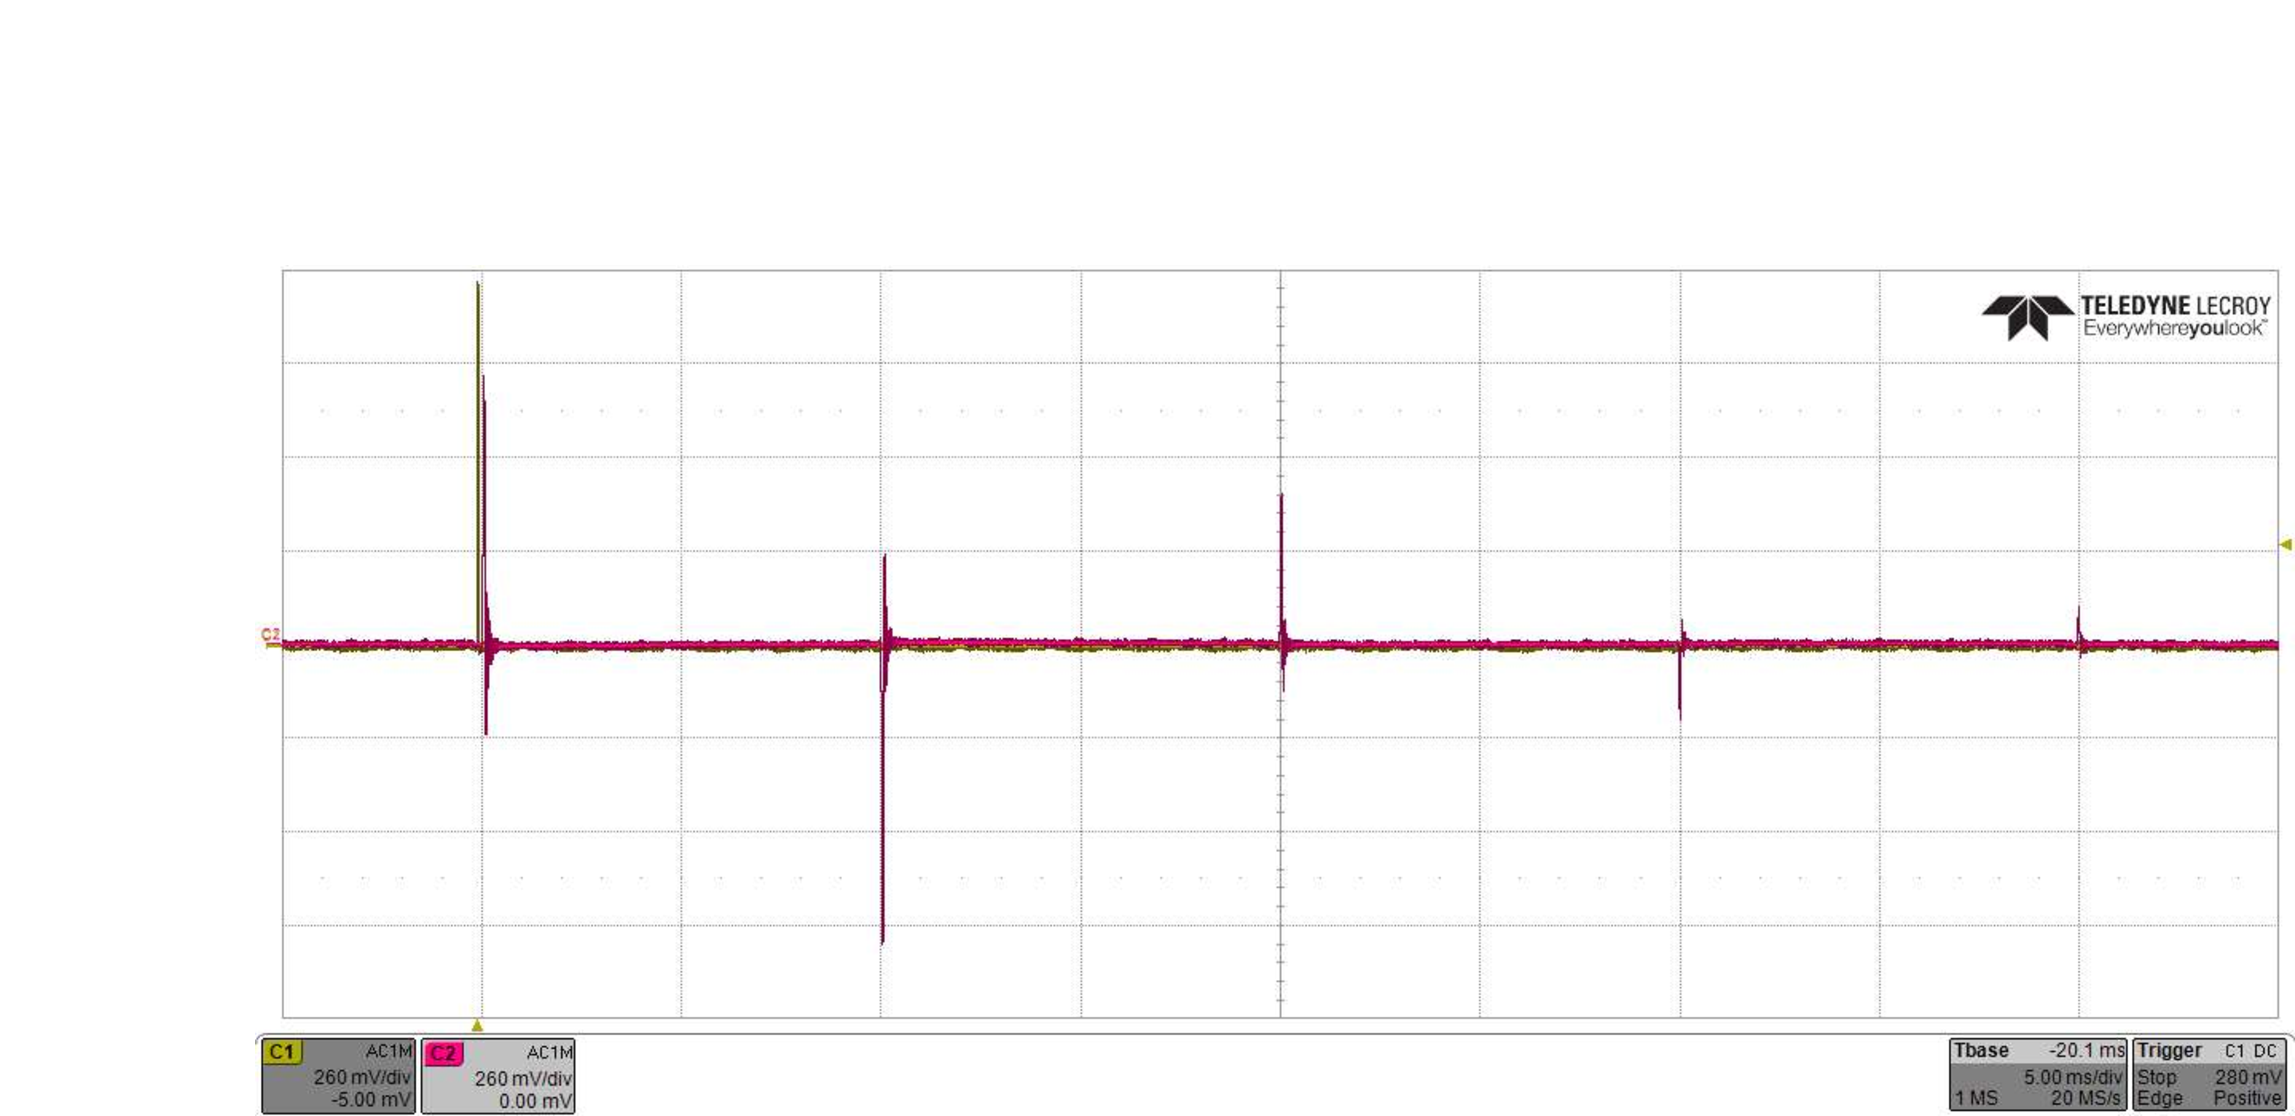
\includegraphics[width=0.9\textwidth, height=5cm]{billeder/reverb.png}
		\caption{Impulsrespons for reverbtesten.}
	\end{minipage}\hfill
	\begin{minipage}{0.50\textwidth}
		\centering
		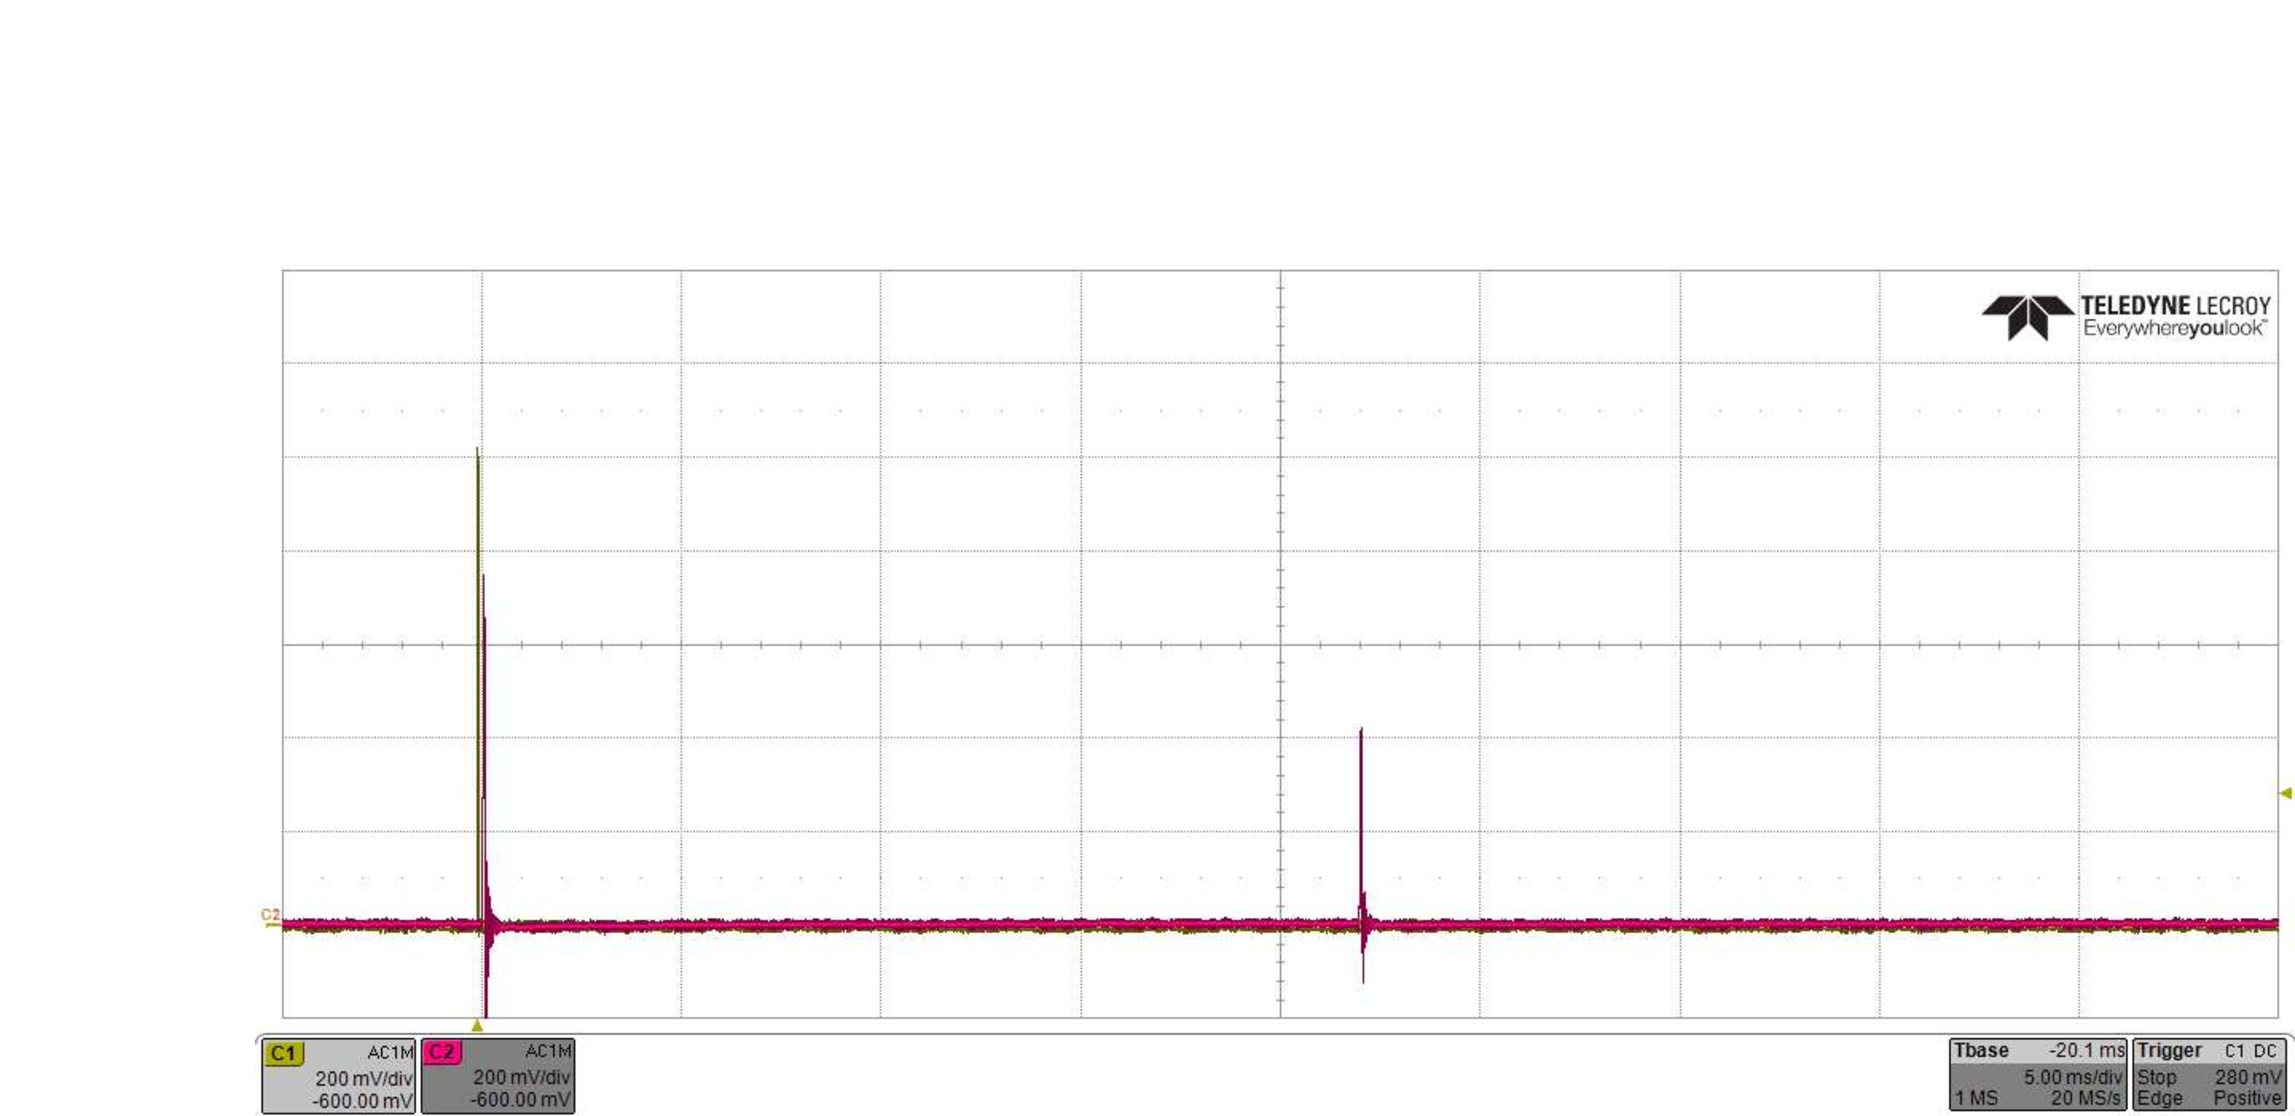
\includegraphics[width=0.9\textwidth, height=5 cm]{billeder/echo.png}
		\caption{Impulsrespons for echoeffekten.}
	\end{minipage}
\end{figure}
På figurene kan det aflæses at delay tiderne stemmer meget præcist overens med de fra programmets side forventede delay tider. På figuren for echo ses også at gentagelsen af impulsen er faldet til ca $400\si{mV}$ hvor det oprindelige output er lige under $800\si{mV}$, hvilket stemmer nogenlunde overens med det forventede gain på $0.5$.\newline 
På reverb figuren ses det at den første gentagelse af impulsen er af samme størrelse som det oprindelige output dette skyldes at feedforward har en gain på $0.5$ og feedback har samme gain så de udgør til sammen en fuld kopi af det oprindelige signal. 
Under normal brug vil disse gains være betydeligt lavere hvilket vil give et noget hurtigere aftagende respons men for at få et tydeligere test resultat blev disse ret høje gain værdier valgt.
%\husk{Sonny}{kan godt huske noget om at vi også testede på indgange til µControlleren, men var der ikke den samme støj på den almindelige indgang og vi ser den næsten heller ikke i matlab plottende}
%Støjen på indgangen skyldes de tre anti-aliasing filtre, som var forbundet via \husk{hvad kalder man de ting} hvilket giver en dårlig forbindelse.\newline
%
%\husk{Sonny}{Først målte tal så hvad de tilsvare præcis i "samples" og så kan der siges at det passer til det delay vi forventede}
%Her \ref{fig:impulsresponsreverb} ses impulsresponset af reverbeffekten.
%Som det fremgår af figuren bliver samplen gengivet med en dæmpning hver $2000$. sample.
%Gains samt delay var sat højt for at overdrive og tydeliggøre feedbacket.\newline
%Som det ses på figuren bliver impulsen feedbacket èn gang som svarende til et ekko efter $2000$ svarende til $45,35\si{mS}$.

